\section{Benutzeroberfläche}
\label{sec:Benutzeroberfläche}

\subsection*{(Anna Kupfer)}

Dieser Abschnitt beschäftigt sich mit der grundlegenden Gestaltung der Benutzeroberfläche für die unterschiedlichen Nutzer [vgl. \cite{UniRos12b}, \cite{UniRos12c}, \cite{balz1996} \cite{Balzert09}, \cite{Schae12}, \cite{Jurij07}]. Zunächst werden allgemeine Anforderungen definiert worauf spezifische zum Bildschirm- und Drucklayout sowie der Tastaturbelegung folgen. Das Kapitel schließt mit einer ausführlichen Betrachtung der Dialogstruktur und untermalt diesen Punkt mit Screenshots zum ersten GUI-Prototypen.\\


\begin{tabular}{p{1.5cm}p{14.5cm}}
 /B10/	& Fensterlayout, Dialogstruktur und Mausbedienung entsprechen dem Windows-Gestaltungs-Regelwerk [vgl. \cite{microsoft1995windows}]. \\[0.25cm]	 
\end{tabular}

\begin{tabular}{p{1.5cm}p{14.5cm}}
 /B11/	& Sämtliche Daten sind passwortgeschützt und dürfen nur von autorisierten Mitarbeitern des Lehrstuhls bearbeitet werden. \\[0.25cm]	 
\end{tabular}


\subsection{Bildschirmlayout}

\begin{tabular}{p{1.5cm}p{14.5cm}}
 /B20/	& Eine übersichtliche Gestaltung der Funktionen und intuitive Nutzung durch ein angepasstes Bildschirmlayout soll vorherrschen. \\[0.25cm]	 
\end{tabular}	

\begin{tabular}{p{1.5cm}p{14.5cm}}
 /B30/	& Standardmäßig startet das Programm mit einer Suchmaske. Weitere Funktionen sind via Tabs und einem Login erreichbar. \\[0.25cm]	 
\end{tabular}

\begin{tabular}{p{1.5cm}p{14.5cm}}
 /BF40/	& Individuelle Anpassungsfähigkeit des Bildschirmlayouts an die Fenstergröße sollte möglich sein. \\[0.25cm]	 
\end{tabular}

\subsection{Drucklayout}

\begin{tabular}{p{1.5cm}p{14.5cm}}
 /B50/	& Nicht angemeldete Nutzer können über die Auswahl verschiedener Lehrveranstaltungen einen Stundenplan im PDF-Format in Din-A4 Größe erzeugen lassen [siehe Abbildung \ref{img:stundenplanAlle}]. \\[0.25cm]	 
\end{tabular}

\begin{tabular}{p{1.5cm}p{14.5cm}}
 /B60/	& Die Hausverwaltungsnutzer können Raumpläne im PFD-Format in Din-A4 Größe erzeugen lassen (ähnlich der Studenten-, Dozenten-, und Lehrstuhlstundenpläne). \\[0.25cm]	 
\end{tabular}

\begin{tabular}{p{1.5cm}p{14.5cm}}
 /B70/	& Mitarbeiter der Lehrstühle können personen- oder lehrstuhlbezogene Wochenpläne in einem PDF-Format in Din-A4 Größe exportieren[siehe Abbildungen \ref{img:StundenplanDoz}, \ref{img:LehrstuhlplanDoz}]. \\[0.25cm]	 
\end{tabular}

Hier einige Beispiele zur Ausgabe des Stundenplans für Studenten, Dozenten und Lehrstühle:
\begin{figure}[H]
\begin{center}
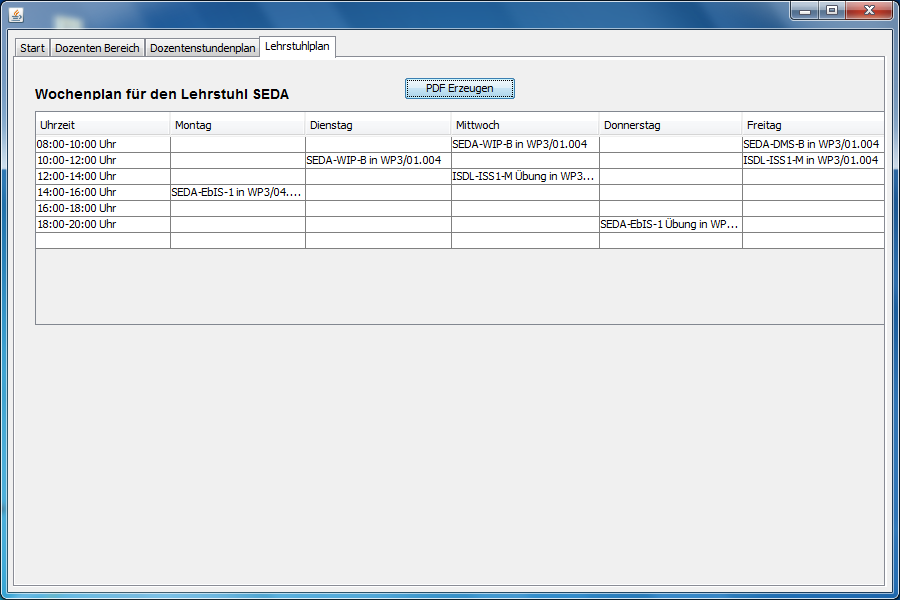
\includegraphics[width=150mm]{images/section_7/DozentenLehrstuhlplan.PNG}
\caption{Lehrstuhlplan}
\label{img:LehrstuhlplanDoz}
\end{center}
\end{figure}

\begin{figure}[H]
\begin{center}
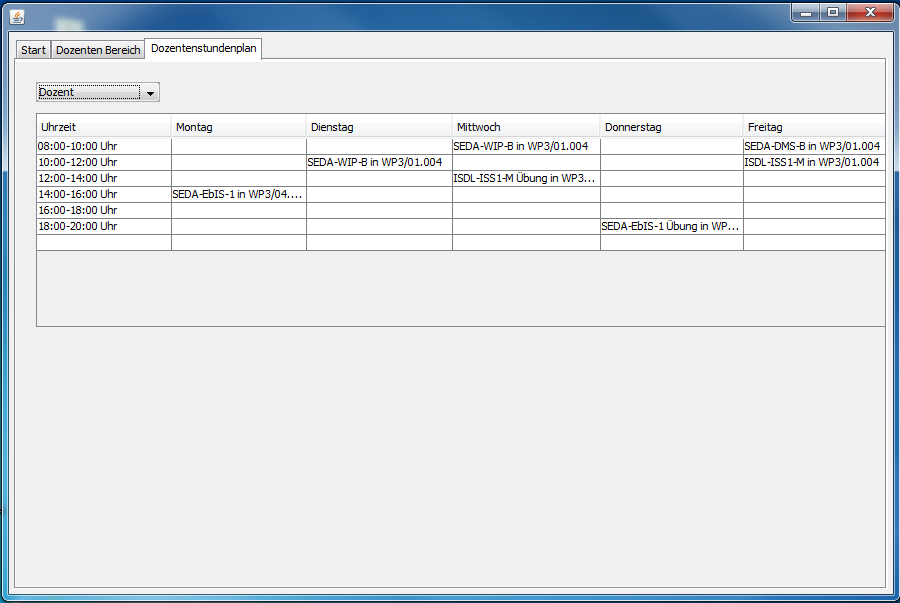
\includegraphics[width=150mm]{images/section_7/DozentenStundenplan.PNG}
\caption{Dozentenstundenplan}
\label{img:StundenplanDoz}
\end{center}
\end{figure}

\begin{figure}[H]
\begin{center}
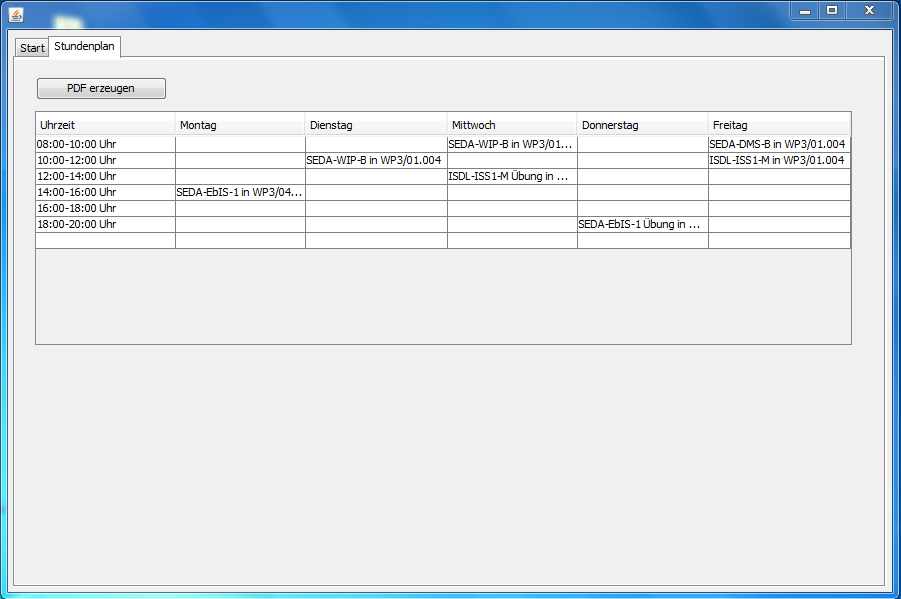
\includegraphics[width=150mm]{images/section_7/HauptseiteAlleStundenplan.PNG}
\caption{Stundenplananzeige, rollenunabhängig}
\label{img:stundenplanAlle}
\end{center}
\end{figure}
 
\subsection{Tastaturbelegung}

\begin{tabular}{p{1.5cm}p{14.5cm}}
 /B80/	& Die Benutzeroberfläche ist auf eine Bedienung mittels Tastatur und Maus auszulegen. Benutzer in der Studentenrolle können keine Eingaben mittels der Tastatur vornehmen. Dozenten und die Hausverwaltung benötigen die Tastatur um verschiedene Funktionen auszuführen. \\[0.25cm]	 
\end{tabular}

\begin{tabular}{p{1.5cm}p{14.5cm}}
 /BF81/	& Mögliche individuelle, nicht dem Windows Standard entsprechende, Tastaturbelegungen sind ein mögliches  Wunschkriterium. \\[0.25cm]	 
\end{tabular}


\subsection{Dialogstruktur}

\begin{tabular}{p{1.5cm}p{14.5cm}}
 /B90/	& Zu Beachten ist: ISO 9241-10: 1996 bzgl. der ergonomischen Anforderungen für Bürotätigkeiten mit Bildschirmgeräten, Teil 10: Grundsätze der Dialoggestaltung. \\[0.25cm]	 
\end{tabular}

\begin{tabular}{p{1.5cm}p{14.5cm}}
 /B91/	& Folgende Rollen sind zu unterscheiden: \\[0.25cm]	 
\end{tabular}\\


\begin{table}[H]
\begin{tabular}{l|l}
Rolle&Rechte\\
\hline
\hline
Student & (F01), F60 , FW61, F130 \\
\hline
Dozent & F01, F20, FW21, F30, F70, F140, F150  \\
\hline
Verwaltungsangestellter & F01, F10, FW21, F40, F50, F51, F80, F90,  \\
\hline
Alle & F01, F100, F110, F120
\end{tabular}
\end{table}
% line
%line

Nachfolgend wird die Dialogstruktur durch den GUI-Prototypen verdeutlicht, um die Benutzeroberfläche vorzustellen und zu erläutern.
Im Anschluss an den Programmstart erscheint die Startseite des UnivIS 2.0 [siehe Abbildung \ref{img:hauptseite}]. Hier können unangemeldete Nutzer (vor allem Stundenten) über Dropdown Menüs verschiedene Lehrveranstaltungen suchen und diese anschließend mittels dem "`+"'-Button die Lehrveranstaltungen zur Stundenplan-Sammlung hinzufügen  [siehe /F60/]. Schon bei der ersten Verwendung des "`+"'-Buttons öffnet sich ein neuer Tab, in welchem der Stundenplan gemäß der selektierten und gesammelten Lehrveranstaltungen ausgegeben wird. Anhand der Radiobuttons (Lehrveranstaltungen und Räume) können gleichzeitig Belegungen einzelner Räume selektiert und weiterhin im Stundenplan-Tab visualisiert werden [siehe /F100/, /F130/].
Im linken Bereich der Benutzeroberfläche befindet sich der Live-Ticker [siehe /F110/], über welchem anstehende Lehrveranstaltungen oder sonstige Informationen ausgegeben werden.
Im unteren linken Bereich befindet sich der Login [siehe /F01/] für Dozenten und die Hausverwaltung (evtl. auch einmal für Studenten) [siehe /FW61/] mittels Benutzerkennung/name und Passwort.
Im Falle einer erfolgreichen Anmeldung als Hausverwaltungsmitglied folgt die Startseite für Hausverwaltungsmitarbeiter [siehe Abbildung \ref{img:hauptseiteVerwaltung}]. 
Sie haben einen unmittelbaren Überblick über alle Raumanfragen und können diese sogleich bearbeiten (freigeben, ablehnen oder etwaige Konflikte lösen) [siehe /F80/, /F40/].
Im linken Bereich bleibt Platz für einen personalisierten Live-Ticker. Weiter unten können die Benutzer auf weitere Aktionen zugreifen.
Werden weitere Aktionen ausgeführt gelangt der Benutzer zu weiteren Listen und kann jeweils Lehrstühle, Nutzer und Räume verwalten (hinzufügen, bearbeiten oder löschen) [siehe /F10/, /F50/, /F51/, /F90/, /F100/ und siehe Abbildungen \ref{img:LehrstuhlVerw} und \ref{img:NutzerVerw}]. Bei der Raumverwaltung kann zusätzlich ein Raumplan erstellt werden [siehe /F120/ und siehe Abbildung \ref{img:RaumVerw}].
Eine letzte abdingbare Funktion wäre die Bearbeitung des LiveTickers um bspw. Dozenten verwaltungstechnische Nachrichten anzeigen lassen zu können [siehe /FW21/].
\begin{figure}[H]
\begin{center}
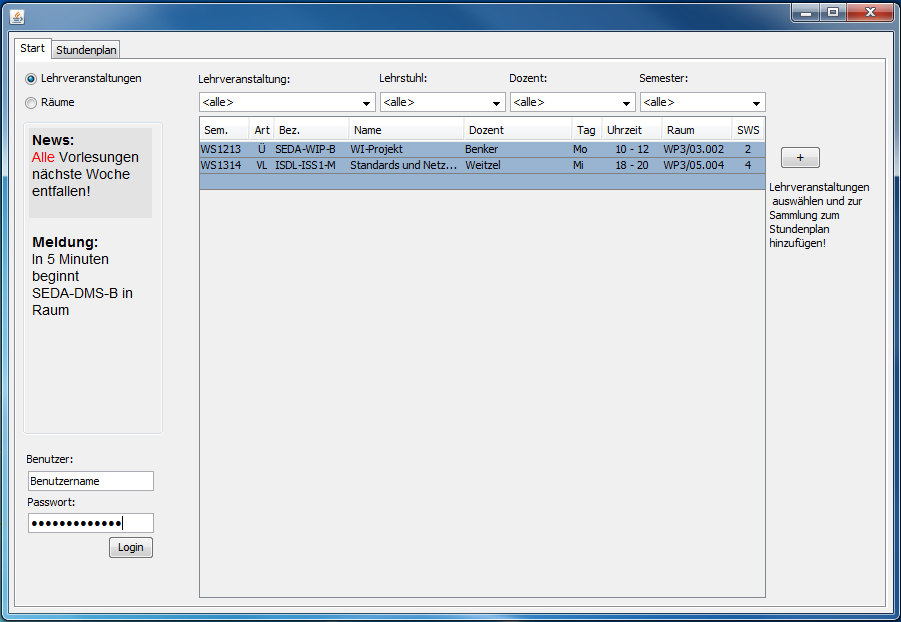
\includegraphics[width=150mm]{images/section_7/HauptseiteAlle.PNG}
\caption{GUI Startseite, rollenunabhängig}
\label{img:hauptseite}
\end{center}
\end{figure}


\begin{figure}[H]
\begin{center}
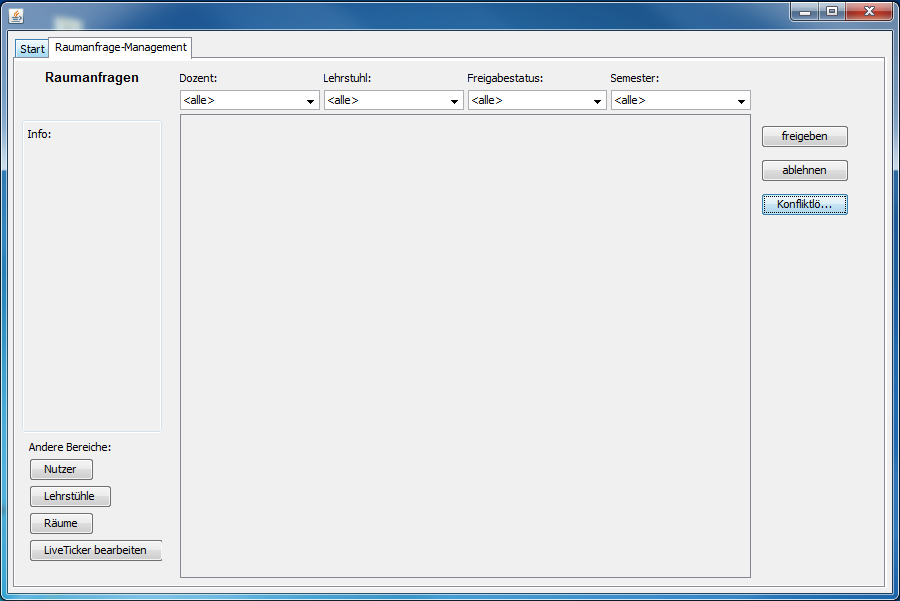
\includegraphics[width=150mm]{images/section_7/VerwaltungHauptseite.PNG}
\caption{Startseite für authentifizierte Benutzer der Hausverwaltung}
\label{img:hauptseiteVerwaltung}
\end{center}
\end{figure}

\begin{figure}[H]
\begin{center}
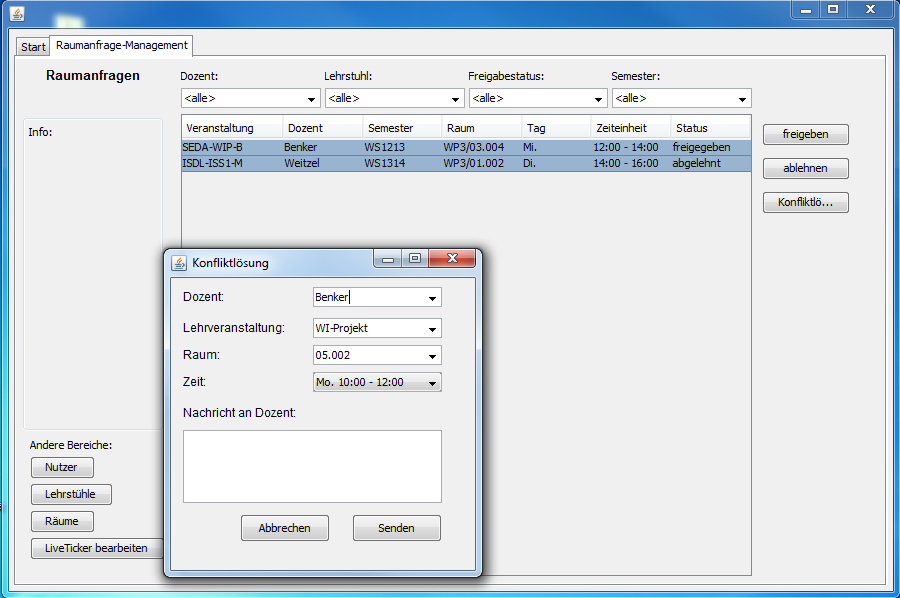
\includegraphics[width=150mm]{images/section_7/VerwaltungRaumanfragen.PNG}
\caption{Konfliktlösung der Raumanfragen}
\label{img:KonfliktlösungVerwaltung}
\end{center}
\end{figure}

\begin{figure}[H]
\begin{center}
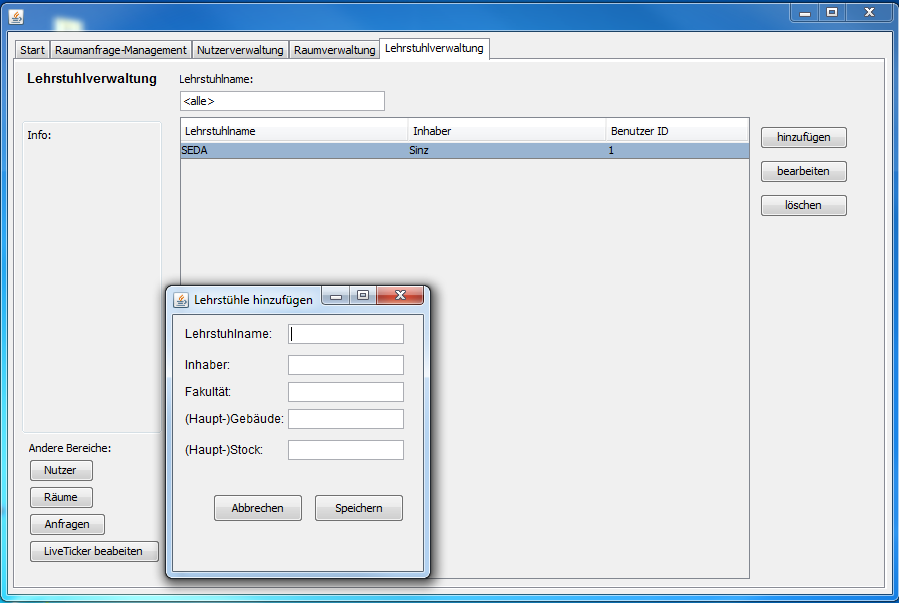
\includegraphics[width=150mm]{images/section_7/VerwaltungLehrstuhlverwaltung.PNG}
\caption{Verwaltung der Lehrstühle}
\label{img:LehrstuhlVerw}
\end{center}
\end{figure}

\begin{figure}[H]
\begin{center}
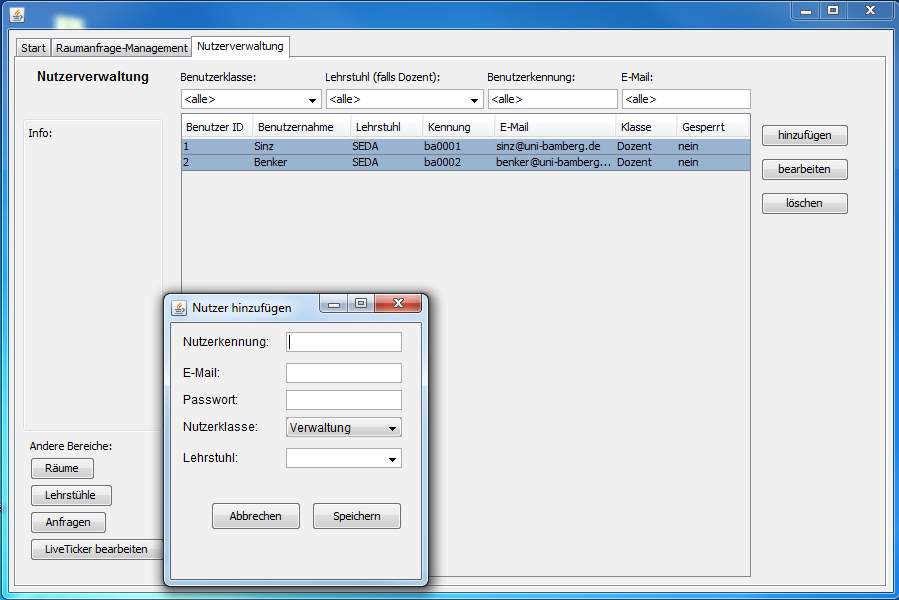
\includegraphics[width=150mm]{images/section_7/VerwaltungNutzerverwaltung.PNG}
\caption{Verwaltung der Nutzer}
\label{img:NutzerVerw}
\end{center}
\end{figure}

\begin{figure}[H]
\begin{center}
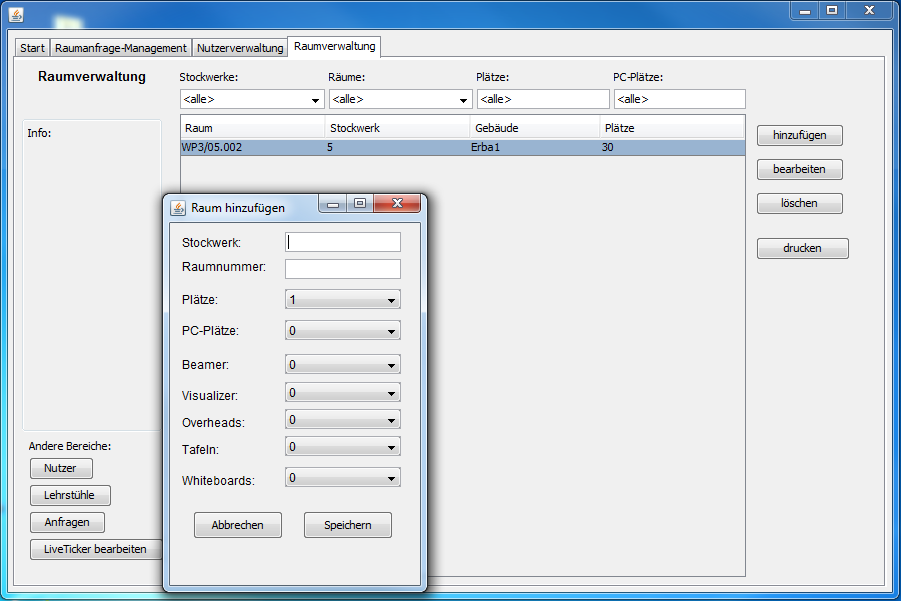
\includegraphics[width=150mm]{images/section_7/VerwaltungRaumverwaltung.PNG}
\caption{Verwaltung der Räume}
\label{img:RaumVerw}
\end{center}
\end{figure}


Die personalisierte Startseite der Dozenten beinhaltet zwei Listen [siehe Abbildung \ref{img:StartDoz}]. In der oberen werden alle Veranstaltungen visualisiert und können nach Lehrstühlen, Dozenten und Semester gefiltert werden. Außerdem wird der Veröffentlichungsstatus sowie die erfolgreich Raumanfrage angezeigt[siehe /F70/]. Eine weitere Liste gibt zusätzliche Auskunft zum Status der Raumanfragen/Raumzuordnungen. Bei einer erfolgreich durchgeführten Raumanfrage kann der jeweilige Dozent seine Lehrveranstaltung anschließend veröffentlichen. Die mit der Raumanfrage bezogenen Nachrichten der Hausverwaltung werden im Live-Ticker (links) angezeigt.
Um Lehrveranstaltungen zunächst überhaupt hinzuzufügen wird der Button "`hinzufügen"' gewählt und in einem neuen Fenster können Lehrstuhl und Dozent ausgewählt werden und somit die Bezeichnung neuer Veranstaltungen gesetzt werden [siehe /F20/ und siehe Abbildung \ref{img:LehrveranstaltungsVerwDoz}]. 
Um der Lehrveranstaltung einen Raum zuzuordnen, kann eine Raumanfrage über den Button "`Raumanfrage"' [siehe Abbild \ref{img:RaumanfrageDoz}] spezifiziert und versandet werden [siehe /F30/]. Hierfür kann entweder ein gewünschter Raum oder nur die besonderen Anforderungen an die Hausverwaltung zur weiteren Bearbeitung übermittelt werden.
Außerdem können die Aktionen eigener Stundenplan [siehe /F150/ und siehe Abbildung \ref{img:StundenplanDoz}] und Lehrstuhlplan [siehe /F140/ und siehe Abbildung \ref{img:LehrstuhlplanDoz}] sowie eine LiveTicker Bearbeitung (um bspw. Studenten veranstaltungs- oder lehrstuhlsbezogene Nachrichten anzeigen lassen zu können) [siehe /FW21/] gewählt werden.


\begin{figure}[H]
\begin{center}
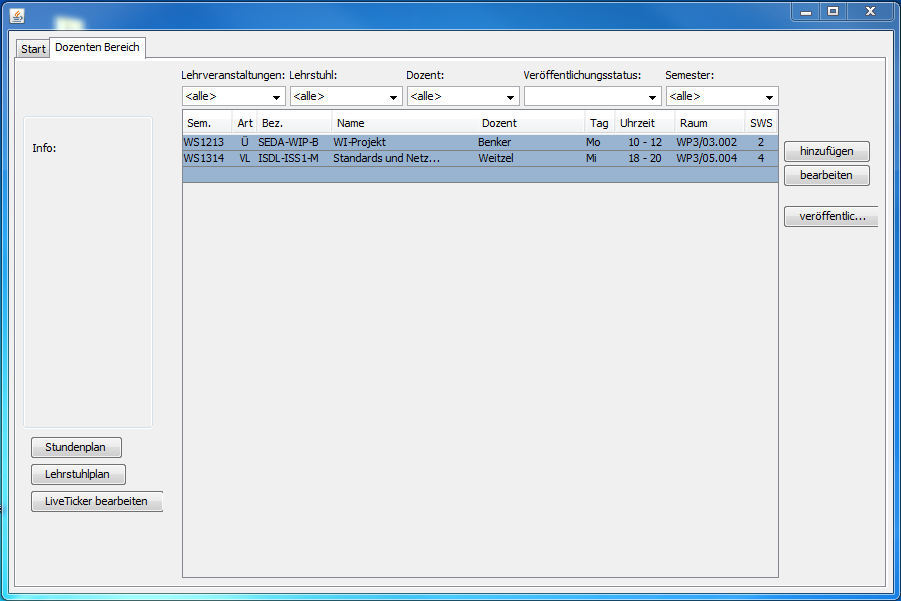
\includegraphics[width=150mm]{images/section_7/DozentenHauptseite.PNG}
\caption{Startseite für Dozenten}
\label{img:StartDoz}
\end{center}
\end{figure}



\begin{figure}[H]
\begin{center}
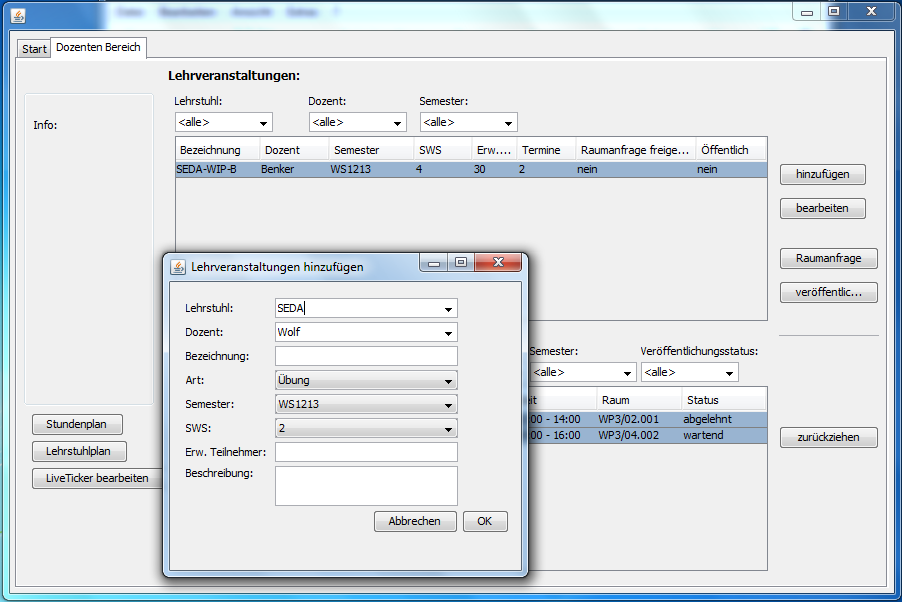
\includegraphics[width=150mm]{images/section_7/DozentenLehrveranstaltungenHinzufuegen.PNG}
\caption{Verwaltung der Lehrveranstaltungen durch die Dozenten}
\label{img:LehrveranstaltungsVerwDoz}
\end{center}
\end{figure}



\begin{figure}[H]
\begin{center}
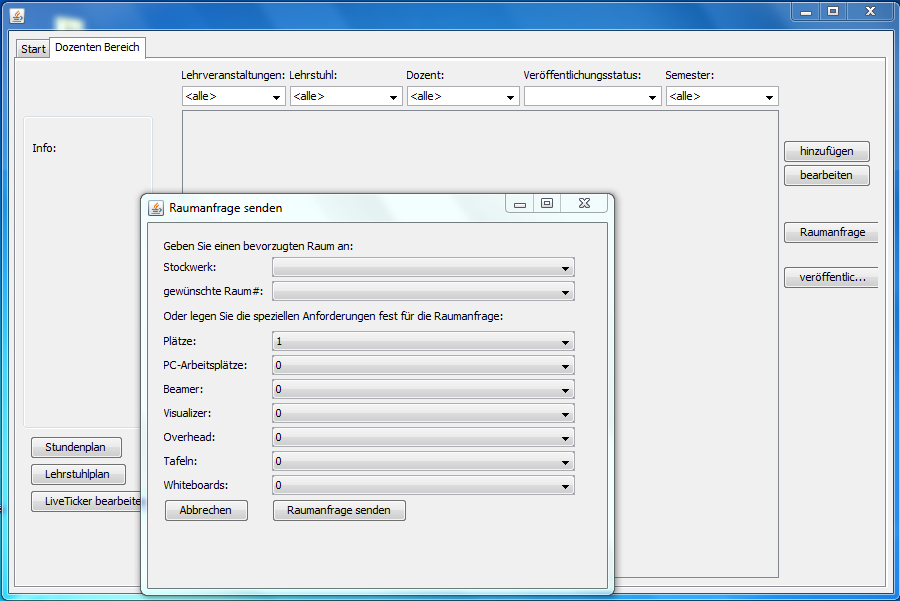
\includegraphics[width=150mm]{images/section_7/DozentenRaumanfrage.PNG}
\caption{Raumanfragen durch die Dozenten}
\label{img:RaumanfrageDoz}
\end{center}
\end{figure}

